\documentclass[a4paper, 11pt]{article}
\usepackage[letterpaper,margin=0.8in]{geometry}
\usepackage{blindtext}
\usepackage{lastpage}
\usepackage{fancyhdr}
\usepackage{xcolor}
\usepackage{setspace}
\usepackage{amsmath}
\usepackage{graphicx}
\usepackage{matlab-prettifier}
\usepackage{float}
\usepackage{multirow}
\definecolor{codemagenta}{rgb}{1,0,0.5}
\definecolor{codegray}{rgb}{0.4,0.4,0.4}
\definecolor{codepurple}{rgb}{0.8,0.2,1}
\definecolor{codeorange}{rgb}{1,0.6,0}
\definecolor{codecyan}{rgb}{0,0.8,1}
\definecolor{codebrown}{rgb}{0.7,0.5,0.3}
\definecolor{codered}{rgb}{1,0.2,0.2}
\definecolor{backcolour}{rgb}{1,1,1}
\lstset{
    language=Python,
    backgroundcolor=\color{backcolour},
    commentstyle=\color{codegray}\itshape,
    keywordstyle=\color{codepurple}\bfseries,
    numberstyle=\tiny\color{codebrown},
    stringstyle=\color{codemagenta}\bfseries,
    basicstyle=\ttfamily\small\color{black},
    emph={True,False,None,self,def,class,return,import,from,as,if,else,elif,for,while,in},
    emphstyle=\color{codepurple}\bfseries,
    emph={[2]np,plt,import,from},
    emphstyle={[2]\color{codeorange}\bfseries},
    breakatwhitespace=false,
    breaklines=true,
    captionpos=b,
    keepspaces=true,
    showspaces=false,
    showstringspaces=false,
    showtabs=false,
    tabsize=4,
    morekeywords={True,False,None}
}
\usepackage[small,bf,hypcap=true]{caption}

\newenvironment{Figure}
  {\par\medskip\noindent\minipage{\linewidth}
   \captionsetup{type=figure}}
  {\endminipage\par\medskip}
\usepackage[hidelinks]{hyperref}
\usepackage{titlesec}
\usepackage{tocloft}

\renewcommand{\cftsecleader}{\cftdotfill{\cftdotsep}}

\graphicspath{{./Figures}}

% Configure the header
\pagestyle{fancy}
\fancyhead[L]{CE 598}
\fancyhead[C]{Coastal \& Harbour Structures Design}
\fancyhead[R]{08/06/2026}

\setlength{\floatsep}{6pt plus 2pt minus 2pt}
\setlength{\textfloatsep}{8pt plus 2pt minus 2pt}
\setlength{\intextsep}{8pt plus 2pt minus 2pt}

\onehalfspacing

\begin{document}

\titleformat{\section}
  {\normalfont\bfseries\fontsize{12}{10}\selectfont}
  {\large\thesection.} 
  {0.3em}
  {}

\thispagestyle{empty}
% -------------------- Title Page --------------------
\begin{titlepage}
    \begin{figure}[H]
        \vspace{0.6cm}
        \centering
        
\includegraphics[width=0.45\textwidth]{logo.png}
    \end{figure}
    \vspace{0.8cm}

    \centering
    \textbf{\LARGE Middle East Technical University}\\[0.3cm]

    \textbf{\LARGE Department of Civil Engineering}\\[0.5cm]

    \textbf{\Large 2025-2026 Spring Semester}\\[1.5cm]

    \textbf{\Large CE598 Coastal \& Harbour Structures Design}\\[0.9cm]

    \textbf{\LARGE Term Project 2}\\[1.5cm]

    \large Instructor:

    \large Dr. Işıkhan Güler\\[1.2cm]

    \large Submitted by:
    
    \large Bilge Kutay
    
    \large 2511798\\[1.5cm]

\end{titlepage}

% -------------------- Table of Contents --------------------
\newpage
\renewcommand{\contentsname}{Table of Contents} 
\begin{center}
    \tableofcontents
\end{center}
\newpage

\listoffigures
\listoftables
\newpage


% -------------------- Introduction --------------------
\section{Introduction}

\hspace*{0.5cm}This report presents the structural design of two cross-sections of a port located in the Filyos region on the Black Sea coast of Turkey. Question 1 selects the deep water design wave properties from the Wave Atlas at point $41.75^{\circ}$N $32.00^{\circ}$E for a return period of 100 years. Question 2 designs cross-section E6 as a composite vertical wall breakwater using the Extended Goda (Takahashi) method, including rubble foundation sizing and stability analysis. Question 3 designs cross-section F1 as a floating concrete pier, covering wave transmission, floating stability, design forces, and mooring line design. Question 4 identifies the forces acting on cross-section E3 and comments on its design procedure. All calculations are performed in MATLAB and the code is provided in the Appendix.

% -------------------- Methodology --------------------
\section{Methodology}

\subsection{Wave Parameters}

\hspace*{0.5cm} The deep water design wave height is obtained from the Wave Atlas at point $41.75^{\circ}$N $32.00^{\circ}$E for a return period of 100 years. Although the Wave Atlas provides a scatter plot of wave period, reliable extraction of $T_p$ was not possible due to significant scatter, and both linear and curve fits yielded unrealistically high values. The deep water peak period is therefore estimated from the limiting steepness $s_0 = H_{s0}/L_0 = 0.04$, giving

\begin{equation}
    T_p = \sqrt{\frac{2\pi H_{s0}}{g \cdot s_0}}
\end{equation}

This is used as input to SWANONE, which yields $H_{m0}$ and $T_p$ at the structure toe after wave transformation. The deep water wavelength and local wavelength at depth $h_s$ are given by

\begin{equation}
    L_0 = \frac{gT_s^2}{2\pi}, \qquad L = L_0 \tanh\left(\frac{2\pi h_s}{L}\right)
\end{equation}

where $T_s = T_p/1.08$ is the significant wave period. The local wavelength is obtained from the gravity wave table.

For the vertical wall breakwater design, the equivalent deep water wave height is $H_0' = K_d K_r H_{s0}$, where $K_d$ and $K_r$ are the diffraction and refraction coefficients. The $\beta$-coefficients for $H_s$ and $H_{max}$ are (Ergin, 2019)

\begin{equation}
    \beta_0 = 0.028\left(\frac{H_0'}{L_0}\right)^{-0.38} e^{20\tan^{1.5}\theta}, \quad \beta_1 = 0.52\, e^{4.2\tan\theta}, \quad \beta_{max} = \max\!\left(0.92,\ 0.32\left(\frac{H_0'}{L_0}\right)^{-0.29} e^{2.4\tan\theta}\right)
\end{equation}

\begin{equation}
    \beta_0^* = 0.052\left(\frac{H_0'}{L_0}\right)^{-0.38} e^{20\tan^{1.5}\theta}, \quad \beta_1^* = 0.63\, e^{3.8\tan\theta}, \quad \beta_{max}^* = \max\!\left(1.65,\ 0.53\left(\frac{H_0'}{L_0}\right)^{-0.29} e^{2.4\tan\theta}\right)
\end{equation}

The significant and maximum wave heights at the toe are then

\begin{equation}
    H_s = \min\!\left(\beta_0 H_0' + \beta_1 h_s,\ \beta_{max} H_0',\ K_s H_0'\right)
\end{equation}

\begin{equation}
    H_{max} = \min\!\left(\beta_0^* H_0' + \beta_1^* h_b,\ \beta_{max}^* H_0',\ 1.8K_s H_0'\right)
\end{equation}

where $h_b = h_s + 5H_s\tan\theta$ is the breaking depth. Two design scenarios are considered using $H_{max}$ and $H_{m0}$ as the design wave height, and results are compared in Section 3.1. For the floating pier design, the wave conditions inside the port are taken directly as $H_i = 1.0$ m and $T = 4.0$ s as specified in the project statement.

\subsection{Vertical Wall Breakwater Design (E6)}

\hspace*{0.5cm} Cross-section E6 is designed as a composite vertical wall breakwater consisting of a concrete caisson seated on a rubble mound foundation. The design follows the Extended Goda (Takahashi) method as presented in Ergin (2019).

\subsubsection{Rubble Foundation Design}

\hspace*{0.5cm} The rubble mound foundation is sized using the Madrigal-Valdes formula (Van der Meer, n.d.)

\begin{equation}
    N_s = \left(5.8\frac{h_1}{h_s} - 0.6\right) N_{od}^{0.19}, \quad 0.5 \leq \frac{h_1}{h_s} \leq 0.8
\end{equation}

where $h_1$ is the water depth at the mound crest, $h_s$ is the total water depth at the toe, and $N_{od} = 0.5$ is the allowable number of displaced armour units per unit width. The median armour stone size, mass, and relative buoyant density are

\begin{equation}
    D_{n50} = \frac{H_{m0}}{N_s \Delta}, \qquad M_{50} = \rho_r D_{n50}^3, \qquad \Delta = \frac{\rho_r - \rho_w}{\rho_w}
\end{equation}

A maximum stone class of 12--15 tonnes is assumed per the project specifications, corresponding to $D_{n50} \leq 1.768$ m. The clear water depth above the armour layer is $d = h_1 - 2D_{n50}$, and the mound berm width $B_M$ is varied between $0.30h_s$ and $0.55h_s$ following the validity range of the formula. The design is optimised by searching all combinations of $h_1/h_s \in [0.50, 0.80]$ and $B_M/h_s \in [0.30, 0.55]$ and selecting the combination that minimises the required caisson width $B$.

\subsubsection{Crest Height}

\hspace*{0.5cm} The minimum crest freeboard $h_c$ is determined from the allowable mean overtopping discharge $q = 10$ l/s/m. The influence of the foreshore is neglected. Based on the EurOtop (2018) classification chart, Equation 7.2 is applied

\begin{equation}
    q = 0.054\sqrt{gH_{m0}^3} \exp\!\left[-\left(\frac{2.12\, h_c}{H_{m0}}\right)^{1.3}\right]
\end{equation}

Rearranging for $h_c$ gives

\begin{equation}
    h_c = \frac{H_{m0}}{2.12} \left[ -\ln\left( \frac{q}{0.054\sqrt{gH_{m0}^3}} \right) \right]^{1/1.3}
\end{equation}

Note that this formula uses $H_{m0}$ regardless of the chosen design wave scenario, as EurOtop formulations are defined in terms of the spectral wave height (EurOtop, 2018).

\subsubsection{Wave Pressure Calculation}

\hspace*{0.5cm} Wave pressures on the caisson are calculated using the Extended Goda (Takahashi) method (Ergin, 2019). The Goda pressure coefficients are

\begin{equation}
    \alpha_1 = 0.6 + \frac{1}{2}\left(\frac{4\pi h_s/L}{\sinh(4\pi h_s/L)}\right)^2, \qquad \alpha_2 = \min\left[\frac{h_b - d}{3h_b}\left(\frac{H_{design}}{d}\right)^2,\ \frac{2d}{H_{design}}\right]
\end{equation}

\begin{equation}
    \alpha_3 = 1 - \frac{h_1}{h_s}\left(1 - \frac{1}{\cosh(2\pi h_s/L)}\right), \qquad \eta^* = 0.75(1+\cos\beta)H_{design}
\end{equation}

The Takahashi impulsive pressure coefficients account for the effects of the rubble mound geometry on wave breaking. The auxiliary parameters are

\begin{equation}
    \delta_{11} = 0.93\left(\frac{B_M}{L} - 0.12\right) + 0.36\left(\frac{h_s-d}{h_s} - 0.6\right), \qquad \delta_{22} = -0.36\left(\frac{B_M}{L} - 0.12\right) + 0.93\left(\frac{h_s-d}{h_s} - 0.6\right)
\end{equation}

\begin{equation}
    \delta_1 = \begin{cases} 20\delta_{11} & \delta_{11} \leq 0 \\ 15\delta_{11} & \delta_{11} > 0 \end{cases}, \qquad \delta_2 = \begin{cases} 4.9\delta_{22} & \delta_{11} \leq 0 \\ 3\delta_{22} & \delta_{11} > 0 \end{cases}
\end{equation}

\begin{equation}
    \alpha_{I1} = \begin{cases} \cosh(\delta_2)/\cosh(\delta_1) & \delta_2 \leq 0 \\ 1/\left(\cosh(\delta_1)\sqrt{\cosh(\delta_2)}\right) & \delta_2 > 0 \end{cases}, \qquad \alpha_{I0} = \min\left(\frac{H_{max}}{d},\ 2\right), \qquad \alpha_I = \alpha_{I0}\cdot\alpha_{I1}
\end{equation}

The modified pressure coefficient is $\alpha^* = \max(\alpha_2,\ \alpha_I)$. The wave pressures are then

\begin{equation}
    p_1 = \frac{1}{2}(1+\cos\beta)\left(\alpha_1 + \alpha^*\cos^2\beta\right)\rho_w g H_{design}, \qquad p_3 = \alpha_3 p_1, \qquad p_u = \frac{1}{2}(1+\cos\beta)\alpha_1\alpha_3\rho_w g H_{design}
\end{equation}

\begin{equation}
    p_2 = \begin{cases} \left(1 - \dfrac{h_c}{\eta^*}\right)p_1 & \eta^* > h_c \\ 0 & \eta^* \leq h_c \end{cases}
\end{equation}

The horizontal force and overturning moment per unit length of the caisson, with respect to the harbour-side base corner, are given by (Ergin, 2019)

\begin{equation}
    F_H = \frac{1}{2}(p_1+p_3)h' + \frac{1}{2}(p_1+p_2)h_c
\end{equation}

\begin{equation}
    M_{FH} = \frac{1}{6}(2p_1+p_3)h'^2 + \frac{1}{2}(p_1+p_2)h'h_c + \frac{1}{6}(p_1+2p_2)h_c^2
\end{equation}

where $h' = d + 2D_{n50}$ is the total submerged height of the caisson.

\subsubsection{Stability Analysis}

\hspace*{0.5cm} The caisson is checked against sliding and overturning failure. The vertical forces per unit length acting on the caisson are (Ergin, 2019)

\begin{equation}
    W = (h_c + h')B\gamma_c, \qquad F_B = h'B\gamma_w, \qquad F_U = \frac{1}{2}p_u B, \qquad M_{FU} = \frac{2}{3}F_U B
\end{equation}

where $\gamma_c$ is the unit weight of concrete and $\gamma_w$ is the unit weight of seawater. The factors of safety against sliding and overturning are

\begin{equation}
    FS_s = \frac{\mu(W - F_B - F_U)}{F_H} \geq 1.2, \qquad FS_o = \frac{(W - F_B)\dfrac{B}{2} - M_{FU}}{M_{FH}} \geq 1.2
\end{equation}

where $\mu = 0.6$ is the friction coefficient. The minimum caisson width $B$ satisfying both criteria is found analytically by rearranging the sliding condition as

\begin{equation}
    B_{slide} = \frac{FS_{req} \cdot F_H}{\mu(W_{unit} - F_{B,unit} - F_{U,unit})}
\end{equation}

and the overturning condition as

\begin{equation}
    B_{overturn} = \sqrt{\frac{FS_{req} \cdot M_{FH}}{\frac{1}{2}(W_{unit} - F_{B,unit}) - \frac{2}{3}p_u}}
\end{equation}

where $W_{unit}$ and $F_{B,unit}$ denote the weight and buoyancy per unit width of the caisson. The design width is $B = \max(B_{slide},\ B_{overturn})$, rounded up to the nearest 0.1 m. The optimum design minimises $B$ over all valid combinations of $h_1/h_s$ and $B_M/h_s$.

\subsection{Floating Pier Design (F1)}

\hspace*{0.5cm} Cross-section F1 is designed as a hollow rectangular concrete floating pier. The design procedure follows the methodology presented in the CE598 floating breakwaters lecture notes, based on OCDI (2002) and PIANC (1994).

\subsubsection{Wave Transmission and Dimensions}

\hspace*{0.5cm} The design wave height inside the port is given as $H_i = 1.0$ m with period $T = 4.0$ s. The maximum design wave height is $H_{max} = 1.8H_i$ (OCDI, 2002). The local wavelength at depth $h = 12$ m is computed from the iterative dispersion relation $L = L_0\tanh(2\pi h/L)$ where $L_0 = gT^2/2\pi$.

The allowable agitation inside the harbour is taken as $H_t = 0.30$ m per the general guideline of OCDI (2002), corresponding to a target transmission coefficient

\begin{equation}
    K_t = \frac{H_t}{H_i} = \frac{0.30}{1.0} = 0.30
\end{equation}

The required pier width $B_{fb}$ is determined by rearranging the Macagno (1953) formula

\begin{equation}
    K_t = \frac{1}{\sqrt{1 + \left(\dfrac{\pi B_{fb} \sinh(kh)}{L\cosh\!\left(\dfrac{2\pi(h-h_d)}{L}\right)}\right)^2}}
    \quad \Rightarrow \quad
    B_{fb} = \frac{L\cosh\!\left(\dfrac{2\pi(h-h_d)}{L}\right)}{\pi\sinh(kh)}\sqrt{\frac{1}{K_t^2}-1}
\end{equation}

The result is independently verified using the Wiegel (1960) formula

\begin{equation}
    K_t = \sqrt{\frac{4\pi(h-h_d)/L + \sinh\!\left(4\pi(h-h_d)/L\right)}{\sinh(4\pi h/L) + 4\pi h/L}}
\end{equation}

The initial draft is assumed as $h_d = 3.0$ m. Since $B_{fb}$ depends on $h_d$ through the Macagno formula, $h_d$ is iteratively updated as $h_d = B_{fb}/3$ until convergence, targeting the upper bound of the recommended ratio $B_{fb}/h_d = 2$--$3$ (WCHL, 1985). The pier length-to-width ratio is also checked against $L_{fb}/B_{fb} < 2.5$ (PIANC, 1988). The wall thickness $t$ of the hollow concrete box is derived from buoyancy equilibrium, requiring the structure weight alone to equal the displaced water weight at draft $h_d$

\begin{equation}
    \gamma_c\left[B_{fb}h_{tot} - (B_{fb}-2t)(h_{tot}-2t)\right] = \gamma_w B_{fb} h_d
\end{equation}

where $h_{tot} = h_f + h_d$ is the total box height and $h_f = 1.0$ m is the assumed freeboard. This equation is quadratic in $t$ and solved analytically.

\subsubsection{Floating Stability}

\hspace*{0.5cm} Three stability conditions are checked following OCDI (2002). The center of buoyancy $B^*$ and center of gravity $G$ are located at $h_d/2$ and $h_{tot}/2$ from the keel respectively, giving a separation of $a = G - B^* = h_f/2$. The metacentric radius and metacentric height are

\begin{equation}
    \rho = \frac{B_{fb}^2}{12h_d}, \qquad GM = \rho - a \geq 0.20 \text{ m}
\end{equation}

For the eccentric loading check, the worst case is a live load of $q = 5.0$ kN/m$^2$ applied to half the pier width, producing a tilting moment $M = q(B_{fb}/2)(B_{fb}/4)$. The resulting tilt angle must satisfy (OCDI, 2002)

\begin{equation}
    \Phi = \frac{M}{\gamma_w V_{sub} \cdot GM} \leq 0.105 \text{ rad} \ (6^{\circ})
\end{equation}

where $V_{sub} = B_{fb} h_d$ is the submerged volume per unit length. The distributed loading stability condition is (OCDI, 2002)

\begin{equation}
    \frac{\gamma_w I}{W} - a > 0
\end{equation}

where $I = B_{fb}^3/12$ is the waterplane moment of inertia per unit length and $W = \gamma_w B_{fb} h_d + q B_{fb}$ is the total weight per unit length including live load. A live load of $q = 5.0$ kN/m$^2$ is used following the standard value for floating piers (OCDI, 2002).

\subsubsection{Design Forces}

\hspace*{0.5cm} The design forces on the floating pier are calculated following OCDI (2002) and PIANC (1994). The transmitted maximum wave height acting on the rear face is $H_t = K_t H_{max}$.

\paragraph{Hydrostatic Wave Forces:} The pressure intensities on the front and rear faces are

\begin{equation}
    p_1 = (H_{max} - h_f)\rho_w g, \quad p_2 = (H_{max} + h_d)\rho_w g, \quad p_3 = \left(h_d + \frac{H_t}{2}\right)\rho_w g, \quad p_4 = p_2 - p_3
\end{equation}

where $p_1 = 0$ when $H_{max} < h_f$. The hydrostatic forces on the front face, rear face, and base are

\begin{equation}
    F_{hf} = \frac{(h_d+h_f)(p_1+p_2)}{2}, \qquad F_{hr} = \frac{\left(h_d - H_t/2\right)p_3}{2}, \qquad F_u = \frac{B_{fb}\,p_4}{2}
\end{equation}

\paragraph{Wave Drift Force:}
\begin{equation}
    F_{wd} = \frac{1}{8}\gamma_w H_i^2 K_r^2 \left(1 + \frac{4\pi h/L}{\sinh(4\pi h/L)}\right)
\end{equation}

\paragraph{Wave Drag and Inertia Forces:} The orbital velocity and acceleration amplitudes at the wave crest elevation are

\begin{equation}
    u_m = \frac{H_{max}}{2}\cdot\frac{gT}{L}\cdot\frac{\cosh\!\left(2\pi(H_{max}/2+h)/L\right)}{\cosh(2\pi h/L)}, \qquad a_x = \frac{H_{max}g\pi}{L}\cdot\frac{\cosh\!\left(2\pi(H_{max}/2+h)/L\right)}{\cosh(2\pi h/L)}
\end{equation}

The drag and inertia forces are computed over one full period and the maximum of their sum is taken as the design value

\begin{equation}
    F_d = C_D h_d \rho_w \frac{u_m^2}{2}, \qquad F_i = C_M A_{sub} \rho_w a_x, \qquad F_{to} = \max_t(F_d + F_i)
\end{equation}

where $C_D = 2.0$, $C_M = 1.5$, and $A_{sub} = B_{fb}h_d$ is the submerged cross-sectional area.

\paragraph{Wind Force:} The wind exposed area is taken as $2h_f$ per unit length to account for rotation of the unit

\begin{equation}
    F_w = C_{DW} \cdot 2h_f \cdot \frac{\rho_{air} u_w^2}{2}
\end{equation}

where $C_{DW} = 2.0$ and $u_w = 12$ m/s.

\paragraph{Current Drag Force:} 

\begin{equation}
    F_{cd} = C_{DC} h_d \rho_w \frac{u_c^2}{2}
\end{equation}

where $C_{DC} = 2.0$ and $u_c = 0.02u_w$. The total horizontal mooring force is

\begin{equation}
    P = (F_{hf} - F_{hr}) + F_{wd} + F_{to} + F_w + F_{cd}
\end{equation}

\subsubsection{Mooring Line Design}

\hspace*{0.5cm} The maximum horizontal and vertical displacements of the floating pier, used to inform the mooring chain length, are taken as the water particle trajectory at the still water level $z = 0$ (OCDI, 2002)

\begin{equation}
    A = \frac{H_{max}}{2}\cdot\frac{\cosh(2\pi h/L)}{\sinh(2\pi h/L)}, \qquad B = \frac{H_{max}}{2}\cdot\frac{\sinh(2\pi h/L)}{\sinh(2\pi h/L)}
\end{equation}

The mooring chain is designed to resist the total horizontal force $P$ acting on one pier unit. The depth below the pontoon bottom is $h_{moor} = h - h_d$. The maximum and minimum projected chain lengths are (OCDI, 2002)

\begin{equation}
    L_{max} = \sqrt{\frac{2Ph_{moor}}{w}}, \qquad L_{min} = -\frac{P\tan\alpha_B}{w} + \sqrt{\left(\frac{P\tan\alpha_B}{w}\right)^2 + \frac{2Ph_{moor}}{w}}
\end{equation}

where $w = 0.5$ kN/m is the submerged chain weight per unit length and $\alpha_B \leq 6^{\circ}$ is the permitted anchor angle (OCDI, 2002). The minimum projected length $L_{min}$ is adopted as the design value. The chain angles at the anchor end ($\theta_1$) and pontoon end ($\theta_2$) are

\begin{equation}
    \theta_2 = \arctan\!\left(\frac{h_{moor}}{L_{min}} + \frac{wL_{min}}{2P}\right), \qquad \theta_1 = \arctan\!\left(\frac{h_{moor}}{L_{min}} - \frac{wL_{min}}{2P}\right)
\end{equation}

The vertical forces at the pontoon and anchor, the maximum chain tension, and the chain sag are

\begin{equation}
    V_b = P\tan\theta_2, \qquad V_a = P\tan\theta_1, \qquad T_{max} = \frac{P}{\cos\theta_2}, \qquad f = \frac{wL_{min}^2}{8P}
\end{equation}

The catenary chain length is computed by numerical integration of

\begin{equation}
    S = \int_0^{L_{min}} \sqrt{1 + \left(\frac{dy}{dx}\right)^2}\,dx, \qquad \frac{dy}{dx} = \frac{V_a + wx}{P}
\end{equation}

\subsection{Composite Wall Forces (E3)}

\hspace*{0.5cm} Cross-section E3 consists of a vertical wall face supported by two concrete blocks with a fill area between them.

The seaward face of the vertical wall is subjected to wave pressures calculated using the Extended Goda (Takahashi) method (Ergin, 2019), identical in formulation to Section 2.2.3. These include the horizontal wave pressure distribution $p_1$, $p_2$, $p_3$, the uplift pressure $p_u$, and the resulting horizontal force $F_H$ and overturning moment $M_{FH}$.

The landward face is subjected to hydrostatic water pressure from the pore water within the fill material and lateral earth pressure from the fill itself. The net horizontal force on the wall is therefore reduced compared to a plain caisson. The vertical forces acting on the wall are the self-weight $W$, buoyancy $F_B$, and wave uplift $F_U$.

The design procedure follows the same sliding and overturning stability checks as Section 2.2.4, with the additional consideration that the fill material contributes both a resisting horizontal pressure and an increased stabilising weight.

% -------------------- Results and Discussion --------------------
\section{Results and Discussion}

\subsection{Vertical Wall Breakwater (E6)}

\hspace*{0.5cm} The 100-year significant wave height is read from the Wave Atlas at point $41.75^{\circ}$N $32.00^{\circ}$E as $H_{s0} = 9.25$ m, as shown in Figure \ref{fig:wave_atlas}. The deep water peak period estimated from the steepness limit $s_0 = 0.04$ is

\begin{equation}
    T_p = \sqrt{\frac{2\pi H_{s0}}{g \cdot s_0}} = \sqrt{\frac{2\pi \times 9.25}{9.81 \times 0.04}} = 12.17 \text{ s}
\end{equation}

This is used as input to SWANONE, which yields $H_{m0} = 8.252$ m and $T_p = 12.448$ s at the structure toe.

\begin{figure}[h]
    \centering
    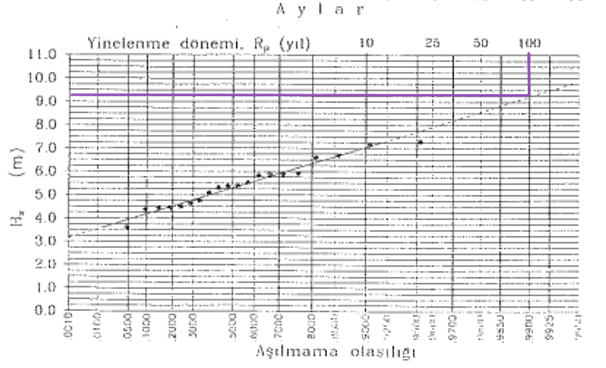
\includegraphics[width=0.7\textwidth]{wave_atlas_hs.png}
    \caption{Significant wave height vs.\ return period from the Wave Atlas at point $41.75^{\circ}$N $32.00^{\circ}$E. The 100-year return period yields $H_{s0} = 9.25$ m (shown by the horizontal line).}
    \label{fig:wave_atlas}
\end{figure}

The random wave breaking formulation yields $H_{max} = 15.359$ m. Since this exceeds the water depth $h_s = 12.0$ m, the Goda beta formula is outside its applicable range for this deep-water site. Accordingly, two design scenarios are evaluated and compared: one using $H_{max}$ from the breaking formulation and one using $H_{m0} = 8.252$ m from SWANONE directly. The local wavelength from the gravity wave table is $L = 115.4$ m.

The key design results for both scenarios are summarised in Table \ref{tab:q2results}.

\begin{table}[H]
\centering
\caption{Vertical wall breakwater design results for both design wave scenarios.}
\label{tab:q2results}
\begin{tabular}{lcc}
\hline
\textbf{Parameter} & \textbf{$H_{design} = H_{max}$} & \textbf{$H_{design} = H_{m0}$} \\
\hline
$H_{design}$ (m) & 15.359 & 8.252 \\
$h_1/h_s$ & 0.70 & 0.80 \\
$B_M/h_s$ & 0.30 & 0.30 \\
$d$ (m) & 5.070 & 6.748 \\
$D_{n50}$ (m) & 1.665 & 1.426 \\
$M_{50}$ (t) & 12.46 & 7.83 \\
$h_c$ (m) & 15.433 & 15.433 \\
$B$ (m) & 20.900 & 8.700 \\
$\alpha_1$ & 0.8914 & 0.8914 \\
$\alpha_2$ & 0.6602 & 0.2957 \\
$\alpha_3$ & 0.8732 & 0.8551 \\
$\alpha^*$ & 0.6602 & 0.2957 \\
$p_1$ (kPa) & 239.621 & 98.500 \\
$p_2$ (kPa) & 79.098 & 0.000 \\
$p_3$ (kPa) & 209.238 & 84.226 \\
$p_u$ (kPa) & 120.203 & 63.244 \\
$F_H$ (kN/m) & 4344.636 & 1486.701 \\
$M_{FH}$ (kN$\cdot$m/m) & 44547.902 & 12687.211 \\
$FS_{sliding}$ & 1.200 & 1.607 \\
$FS_{overturning}$ & 1.937 & 1.324 \\
\hline
\end{tabular}
\end{table}

The $H_{max}$ scenario produces a caisson width of $B = 20.9$ m and pressures exceeding 239 kPa, driven by a design wave height that surpasses the water depth. The $H_{m0}$ scenario yields a more physically consistent design with $B = 8.7$ m. In both cases the crest height $h_c = 15.433$ m exceeds the water depth, which is a consequence of the extreme wave climate at this deep-water site and the EurOtop formula yielding large freeboard requirements for high $H_{m0}$ values.

Note that $p_2 = 0$ in the $H_{m0}$ scenario because the wave run-up $\eta^* = 12.38$ m does not reach the structure crest $h_c = 15.43$ m, meaning no overtopping pressure reduction acts at the top of the caisson.

The cross-sections for both design scenarios are shown in Figures \ref{fig:q2_hmax} and \ref{fig:q2_hm0}.

\begin{figure}[H]
    \centering
    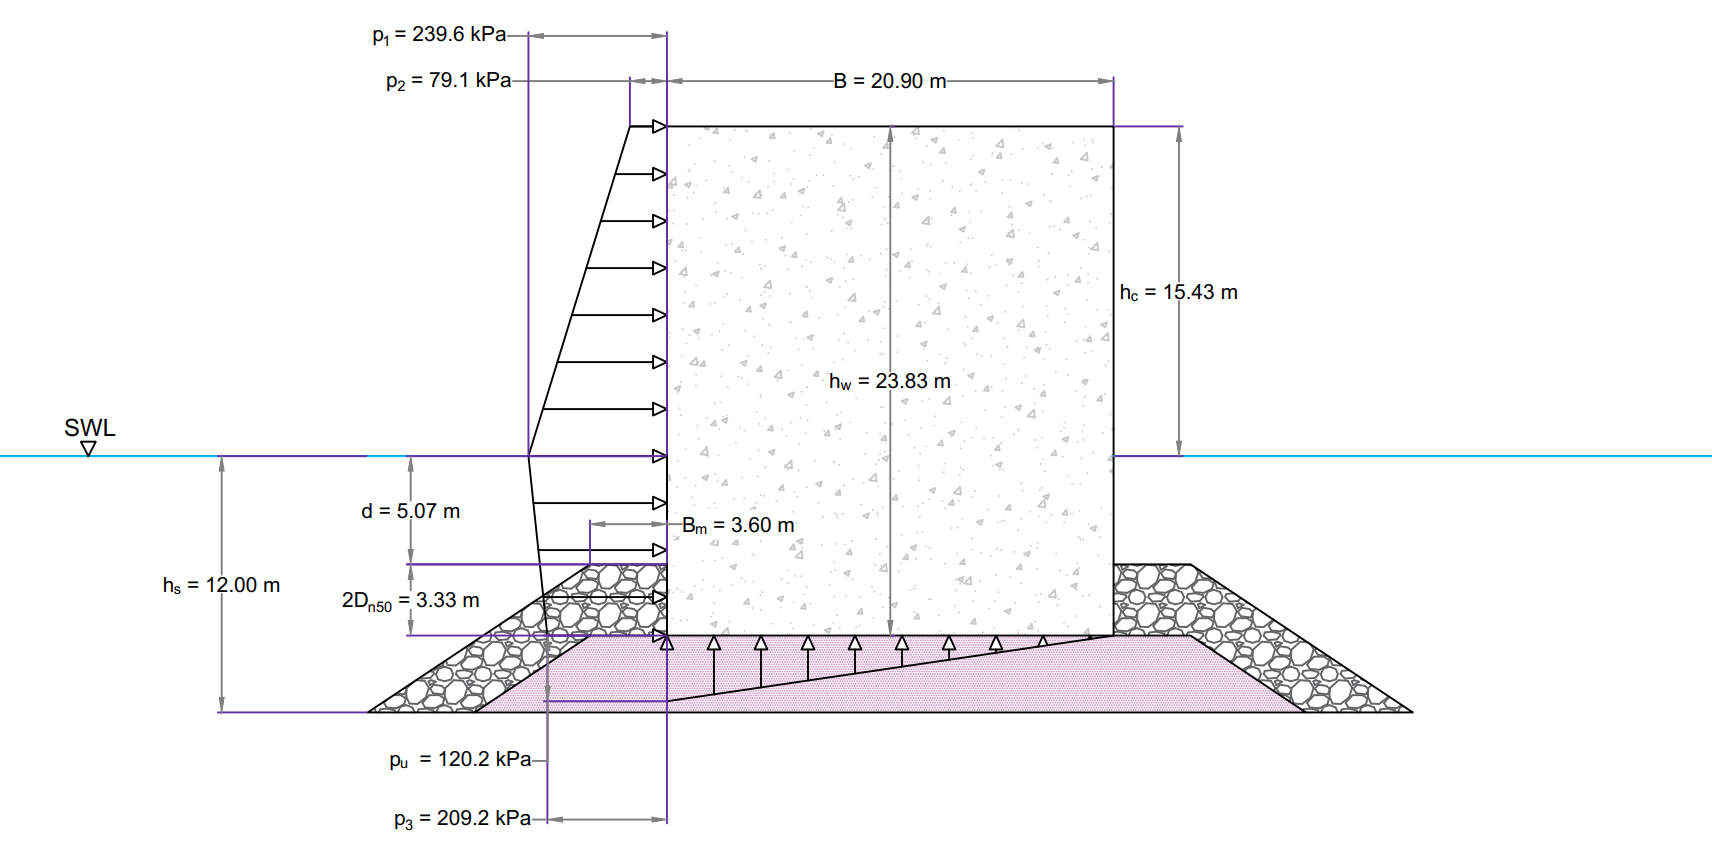
\includegraphics[width=\textwidth]{q2_hmax.png}
    \caption{Vertical wall breakwater cross-section for the $H_{max} = 15.359$ m design scenario ($B = 20.90$ m).}
    \label{fig:q2_hmax}
\end{figure}

\begin{figure}[H]
    \centering
    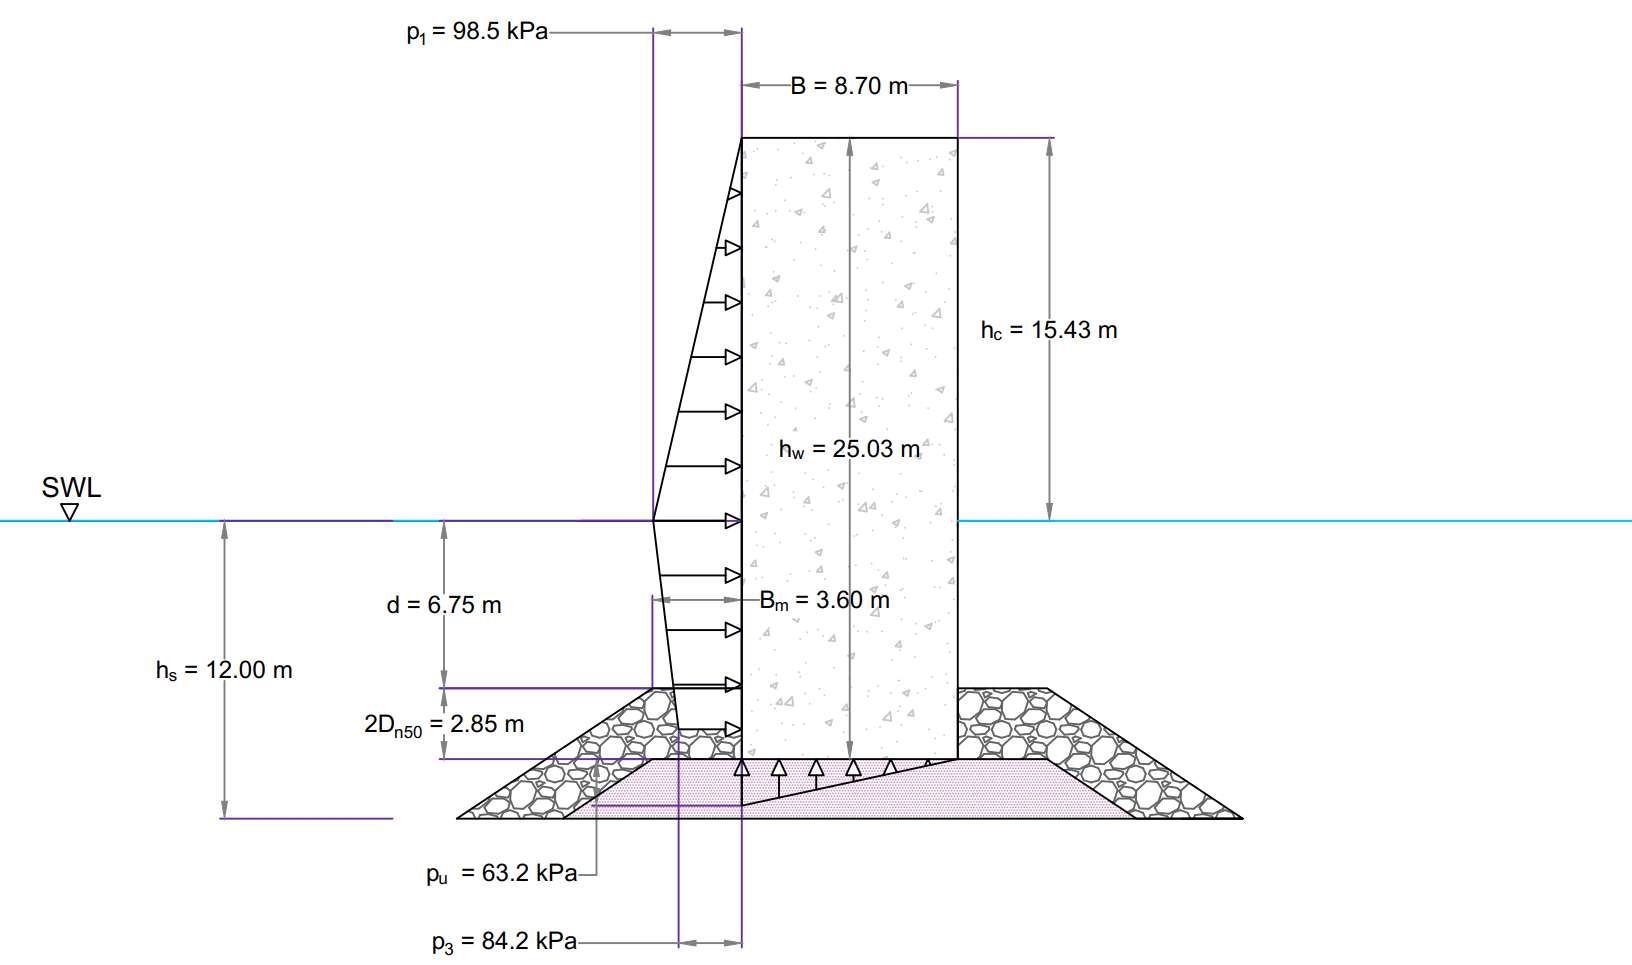
\includegraphics[width=\textwidth]{q2_hm0.png}
    \caption{Vertical wall breakwater cross-section for the $H_{m0} = 8.252$ m design scenario ($B = 8.70$ m).}
    \label{fig:q2_hm0}
\end{figure}

\subsection{Floating Pier (F1)}

\hspace*{0.5cm} The local wavelength at depth $h = 12.0$ m and period $T = 4.0$ s is $L = 24.865$ m. The pier width required to achieve $K_t = 0.30$ converges to $B_{fb} = 10.532$ m with a draft of $h_d = 3.511$ m after iteration. The dimension checks are satisfied with $B_{fb}/h_d = 3.00$ and $L/B_{fb} = 2.36 < 2.5$. The wall thickness from buoyancy equilibrium is $t = 0.580$ m. The Macagno and Wiegel transmission coefficients are $K_{t,Mac} = 0.300$ and $K_{t,Wie} = 0.429$ respectively. The higher Wiegel value is expected as it models a thin vertical barrier rather than a finite-width structure, making it less representative for this case.

The three floating stability checks all pass as shown in Table \ref{tab:q3_stability}.

\begin{table}[h]
\centering
\caption{Floating stability check results for cross-section F1.}
\label{tab:q3_stability}
\begin{tabular}{lccc}
\hline
\textbf{Check} & \textbf{Result} & \textbf{Limit} & \textbf{Status} \\
\hline
$\rho - a$ (m) & 2.133 & $\geq 0.20$ & PASS \\
$\Phi$ (deg) & 4.91 & $\leq 6.00$ & PASS \\
$\gamma_w I/W - a$ (m) & 1.812 & $> 0$ & PASS \\
\hline
\end{tabular}
\end{table}

The design forces are summarised in Table \ref{tab:q3_forces}. The inertia force dominates the orbital wave forces ($F_i = 159.073$ kN/m vs $F_d = 11.420$ kN/m), and the maximum combined force $F_{to} = 159.073$ kN/m occurs at $t = 3T/4$ when acceleration is maximum and velocity is zero, consistent with the note in OCDI (2002) that drag and inertia cannot peak simultaneously.

\begin{table}[h]
\centering
\caption{Design forces for cross-section F1.}
\label{tab:q3_forces}
\begin{tabular}{lc}
\hline
\textbf{Force} & \textbf{Value (kN/m)} \\
\hline
$F_{hf} - F_{hr}$ (net hydrostatic) & 78.470 \\
$F_{wd}$ (wave drift) & 1.317 \\
$F_{to}$ (drag + inertia) & 159.073 \\
$F_w$ (wind) & 0.353 \\
$F_{cd}$ (current) & 0.207 \\
\textbf{Total $P$} & \textbf{239.420} \\
\hline
\end{tabular}
\end{table}

The mooring chain is designed for the total horizontal force $P = 239.420$ kN/m. The maximum and minimum projected lengths are $L_{max} = 90.17$ m and $L_{min} = 52.93$ m, and the minimum length is adopted. The chain makes angles of $\theta_1 = 6.00^{\circ}$ at the anchor end and $\theta_2 = 12.17^{\circ}$ at the pontoon end. The maximum chain tension at the pontoon end is $T_{max} = 244.924$ kN/m with a sag of $f = 0.731$ m and catenary length $S = 53.64$ m. The floating body displacements at still water level are $A = 0.904$ m horizontally and $B = 0.900$ m vertically.

The cross-section and mooring diagrams are shown in Figures \ref{fig:q3_section} and \ref{fig:q3_mooring}.

\begin{figure}[H]
    \centering
    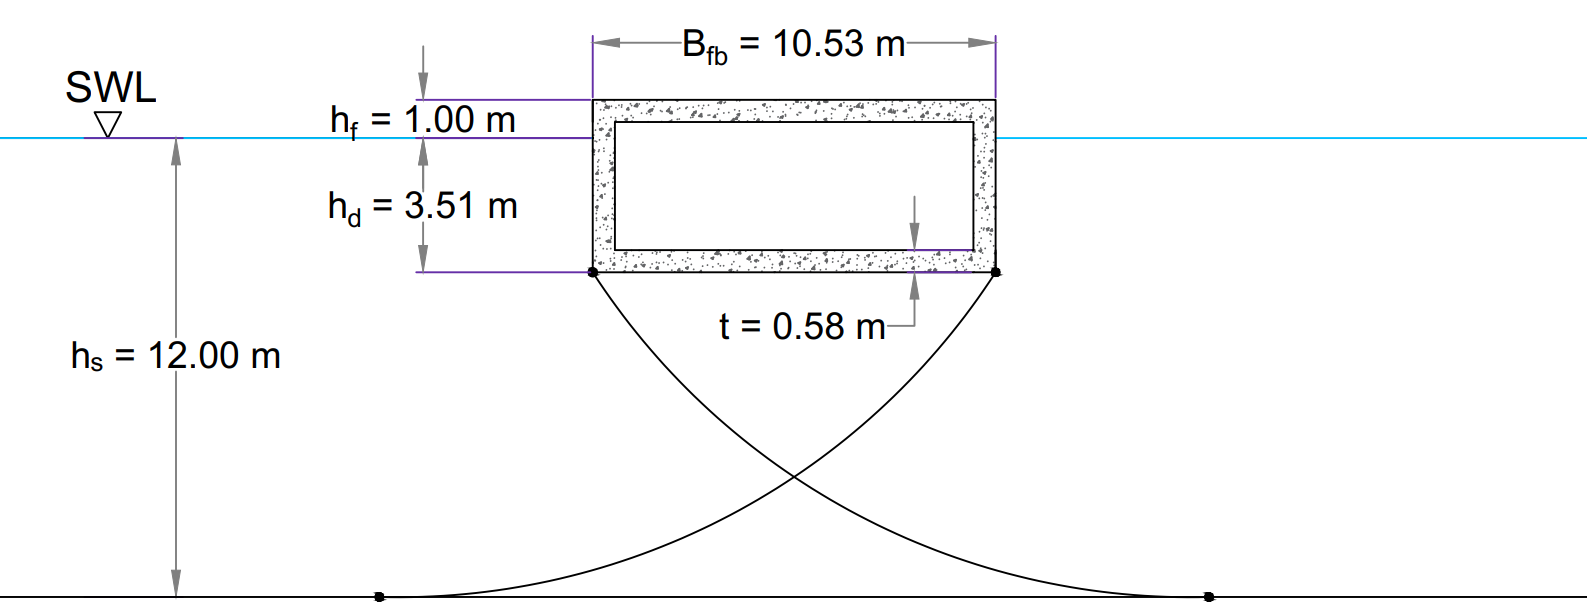
\includegraphics[width=\textwidth]{q3_section.png}
    \caption{Floating pier cross-section showing box dimensions and mooring chain geometry.}
    \label{fig:q3_section}
\end{figure}

\begin{figure}[H]
    \centering
    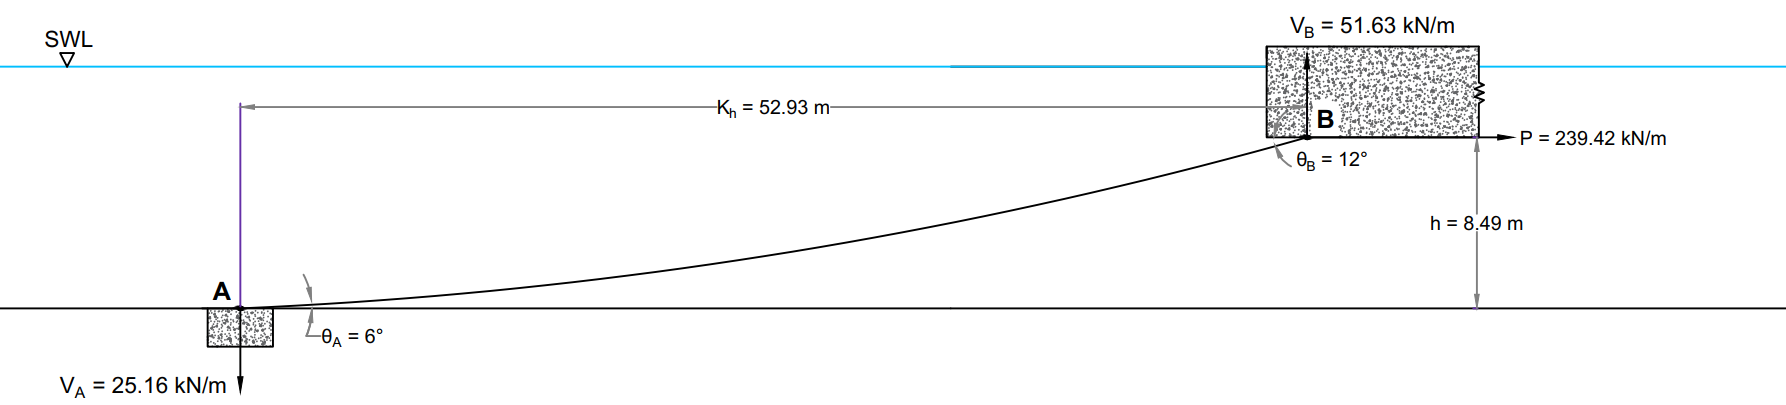
\includegraphics[width=\textwidth]{q3_mooring.png}
    \caption{Mooring line diagram for cross-section F1 showing chain angles, forces, and projected length $K_h = L_{min} = 52.93$ m.}
    \label{fig:q3_mooring}
\end{figure}

\subsection{Composite Wall Forces (E3)}

\hspace{0.5cm}Figure~\ref{fig:E3forces} presents the force system acting on the composite vertical wall at cross-section E3. The force system acting on the E3 cross-section differs from that of a conventional vertical wall breakwater because the wall is backed by a fill area and concrete blocks. The seaward face is subjected to wave-induced pressures represented by the Extended Goda pressure distribution and the associated uplift pressure beneath the wall. These loads generate the primary horizontal force and overturning moment acting on the structure.

On the landward side, the retained fill produces lateral earth pressure acting toward the seaward direction. Depending on the permeability of the fill and the hydraulic conditions within the structure, hydrostatic pressures may also develop within the fill material. These forces oppose the seaward wave loading and therefore contribute to the overall force equilibrium of the wall.

The vertical force system consists of the self-weight of the wall, buoyancy, and uplift pressure. The self-weight provides the principal stabilizing force against sliding and overturning, while buoyancy and uplift reduce the effective stabilizing weight of the structure.

The design procedure for the E3 section therefore follows the conventional methodology for vertical wall breakwaters by evaluating horizontal wave loading, vertical forces, sliding stability, overturning stability, and foundation performance. Additional consideration is given to the interaction between the wall and the retained fill, which influences both the horizontal and vertical force balance acting on the structure.

\begin{figure}[H]
    \centering
    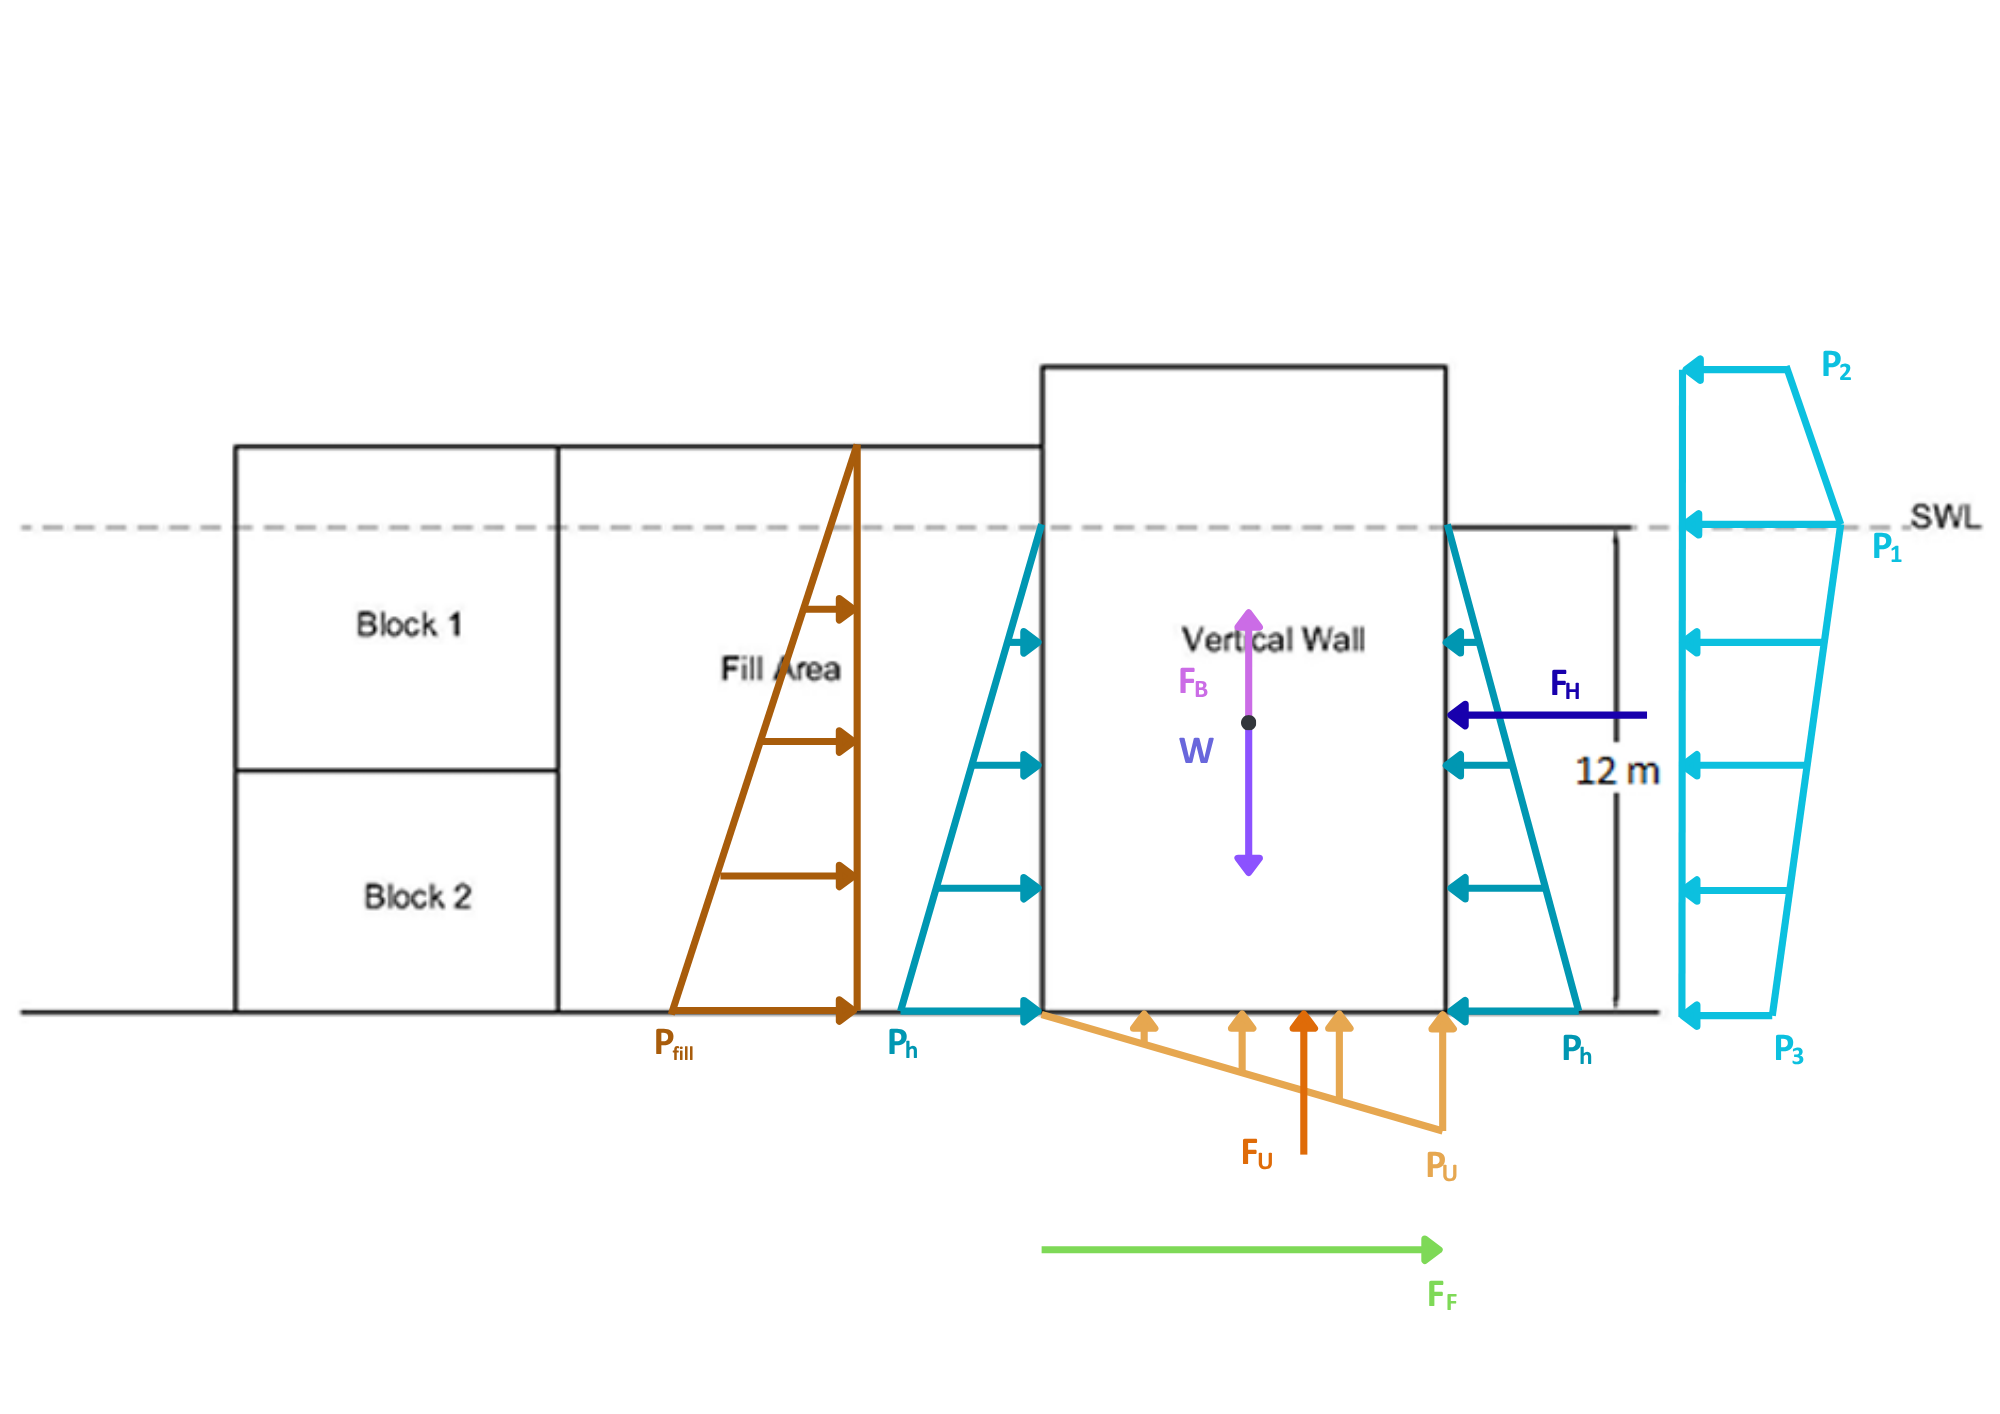
\includegraphics[width=\textwidth]{E3_forces.png}
    \caption{Forces acting on the composite vertical wall at cross-section E3. The seaward face is subjected to the Extended Goda wave pressure distribution ($p_1$, $p_2$, $p_3$) and the resultant horizontal wave force $F_H$. On the landward side, the wall is subjected to lateral earth pressure from the retained fill ($P_{\mathrm{fill}}$) and hydrostatic pressure within the saturated fill ($P_h$). Hydrostatic pressure from the seaward side is also shown. Vertical forces include the self-weight of the wall ($W$), buoyancy force ($F_B$), and uplift force ($F_U$) generated by the pressure distribution $P_u$ beneath the base. The frictional resistance force ($F_F$) acts along the foundation interface and opposes sliding.}
    \label{fig:E3forces}
\end{figure}

\newpage
% -------------------- Conclusion --------------------
\section{Conclusion}
\hspace{0.5cm}This report presented the design and assessment of a vertical wall breakwater, a floating pier, and a composite wall section for the given site conditions.

For the vertical wall breakwater, two design wave scenarios were investigated using the Extended Goda (Takahashi) method. The design based on $H_{max}$ resulted in a significantly larger caisson width and wave pressures, while the design based on $H_{m0}$ produced a more practical and physically realistic structure. In both cases, the required crest freeboard was found to be relatively large due to the severe wave climate at the site.

The floating pier was designed to satisfy the required wave transmission criterion and all stability requirements. The selected dimensions achieved the target transmission coefficient while maintaining adequate metacentric stability and acceptable behaviour under eccentric loading. The mooring system was then sized based on the calculated environmental loads acting on the structure.

Finally, the force system acting on the composite wall section E3 was examined. In addition to the wave pressures acting on the seaward face, the effects of uplift, buoyancy, hydrostatic pressures, and fill-induced earth pressures were identified and discussed. These additional forces influence the overall stability of the wall and must be considered during design.

Overall, the analyses demonstrate how different coastal structures respond to the same environmental conditions and highlight the importance of considering both hydraulic loading and stability requirements when developing safe and effective harbour structures.

\newpage

% -------------------- References --------------------

\begin{thebibliography}{99}
\addcontentsline{toc}{section}{References}

\bibitem{RockManual}
CIRIA, CUR, CETMEF. (2007). \textit{The Rock Manual: The use of rock in hydraulic engineering} (2nd ed.). CIRIA.

\bibitem{}
Ergin, A. (2019). \textit{Coastal engineering}. Middle East 
Technical University.

\bibitem{CE598}
Middle East Technical University, Department of Civil Engineering. (2025). \textit{CE 598 lecture notes} [Course notes].

\bibitem{CE593}
Middle East Technical University, Department of Civil Engineering. (2025). \textit{CE 593 lecture notes} [Course notes].

\bibitem{EurOtop2018}
Van der Meer, J.W., Allsop, N.W.H., Bruce, T., De Rouck, J., Kortenhaus, A., Pullen, T., Sch\"{u}ttrumpf, H., Troch, P., \& Zanuttigh, B. (2018). \textit{EurOtop: Manual on wave overtopping of sea defences and related structures} (2nd ed.). www.overtopping-manual.com.

\end{thebibliography}
\newpage

% -------------------- Appendix --------------------
\appendix
\section{Appendix}

\subsection{MATLAB Code:}
\begin{lstlisting}[frame=single, numbers=left, style=Matlab-Pyglike]
%% ============================================================
%  TERM PROJECT 2 - Q2: VERTICAL WALL BREAKWATER DESIGN (E6)
% ============================================================
clear; clc;
%% --- Input Parameters ---
g       = 9.81;         % gravitational acceleration (m/s^2)
rho_w   = 1.025;        % seawater density (kg/m^3)
rho_c   = 2.400;
rho_r   = 2.700;
Delta   = (rho_r - rho_w) / rho_w;
gamma_r = 2700 * g;     % unit weight of rock (N/m^3)
mu      = 0.6;          % friction coefficient
FS_req  = 1.2;          % required factor of safety (sliding and overturning)
beta    = 0;            % wave angle (deg)
Nod     = 0.5;

% Site parameters
hs      = 12.0;         % water depth at toe (m), TP2 assumption
tan_th  = 0.1;          % foreshore slope (1:10), TP2 assumption

%% --- Wave Parameters ---
Hs0 = 9.25;
Hm0 = 8.252;            % Hm0 from SwanOne (m)
Tp = 12.448;            % peak period from SwanOne (s)
Ts = Tp / 1.08;         % significant wave period (s)
L0 = g * Ts^2 / (2*pi); % deep water wavelength (m)
q_allow = 10e-3;

%% --- Random Wave Breaking Formulation ---
surf = hs / L0;
Ks = 0.993;
Kd = 1;
Kr = 1;
H0_p = Kd * Kr * Hs0;

% Coefficients
beta_0 = 0.028*(H0_p / L0)^-0.38 * exp(20*tan_th^1.5);
beta_1 = 0.52 * exp(4.2*tan_th);
beta_max = max(0.92, 0.32 * (H0_p/L0)^-0.29 * exp(2.4*tan_th));

beta_0_star = 0.052*(H0_p / L0)^-0.38 * exp(20*tan_th^1.5);
beta_1_star = 0.63 * exp(3.8*tan_th);
beta_max_star = max(1.65, 0.53 * (H0_p/L0)^-0.29 * exp(2.4*tan_th));

Hs = min([beta_0*H0_p + beta_1*hs, beta_max*H0_p, Ks*H0_p]);

hb = hs + 5*Hs*tan_th;
surf_max = hb / L0;
Hmax = min([beta_0_star*H0_p + beta_1_star*hb, beta_max_star*H0_p, 1.8*Ks*H0_p]);

use_Hmax = false;

if use_Hmax
    Hdesign = Hmax;
else
    Hdesign = Hm0;
end
fprintf('H_max = %.3f m  |  Hm0 = %.3f m  |  Hdesign = %.3f m\n', Hmax, Hm0, Hdesign)

L = hs/0.104;
eta_star = 0.75*(1+cosd(beta))*Hdesign;
alpha1   = 0.6 + 0.5*(4*pi*hs/L / sinh(4*pi*hs/L))^2;

% --- EurOtop hc Calculation ---
hc = (Hm0 / 2.12) *(-log(q_allow/(0.054*sqrt(g*Hm0^3))))^(1/1.3);

best.B_exact = inf;

for h1_hs = 0.50 : 0.01 : 0.80
    h1 = h1_hs * hs;

    % Madrigal-Valdes
    Ns   = (5.8*h1_hs - 0.6) * Nod^0.19;
    Dn50 = Hm0 / (Ns * Delta);
    M50  = rho_r * Dn50^3;
    Dn50 = Hm0 / (Ns * Delta);
    if Dn50 > 1.768; continue; end

    % depth above mound top
    d = h1 - 2*Dn50;
    if d <= 0; continue; end

    % --- Goda coefficients ---
    alpha2 = min([(hb-d)/(3*hb)*(Hdesign/d)^2,  2*d/Hdesign]);

    hw     = hc + d + 2*Dn50;
    alpha3 = 1 - h1/hs * (1 - 1/cosh(2*pi*hs/L));

    for Bm_hs = 0.30 : 0.01 : 0.55 
        Bm = Bm_hs * hs;

        % Takahashi impulsive coefficient
        d11 = 0.93*(Bm/L - 0.12) + 0.36*((hs-d)/hs - 0.6);
        d22 = -0.36*(Bm/L - 0.12) + 0.93*((hs-d)/hs - 0.6);
        if d11 <= 0; d1 = 20*d11; else; d1 = 15*d11; end
        if d11 <= 0; d2 = 4.9*d22; else; d2 = 3*d22; end
        if d2 <= 0
            aIB = cosh(d2)/cosh(d1);
        else
            aIB = 1/(cosh(d1)*sqrt(cosh(d2)));
        end
        aIH    = min(Hmax/d, 2.0);
        aI     = aIH * aIB;
        alphaX = max(alpha2, aI);

        % --- Pressures ---
        p1 = 0.5*(1+cosd(beta))*(alpha1 + alphaX*cosd(beta)^2)*rho_w*g*Hdesign;
        p3 = alpha3 * p1;
        pu = 0.5*(1+cosd(beta))*alpha1*alpha3*rho_w*g*Hdesign;

        hc_eff = min(hc, eta_star);
        if eta_star > hc
            p2 = (1 - hc/eta_star)*p1;
        else
            p2 = 0;
        end
        
        h_p = d + 2*Dn50;
        % --- Forces and moments ---
        FH  = 0.5*(p1+p3)*h_p + 0.5*(p1+p2)*hc_eff;
        MFH = (1/6)*(2*p1+p3)*h_p^2 + 0.5*(p1+p2)*h_p*hc_eff + (1/6)*(p1+2*p2)*hc_eff^2;

        % --- Stability: find minimum B ---
        % per unit B:
        W_unit  = rho_c * g * (hc + h_p);
        FB_unit = rho_w * g * (h_p);
        FU_unit = 0.5 * pu;

        % sliding
        B_slide = FS_req * FH / (mu*(W_unit - FB_unit - FU_unit));

        % overturning
        coeff = (W_unit - FB_unit)/2 - (2/3)*pu;
        if coeff > 0
            B_overturn = sqrt(FS_req * MFH / coeff);
        else
            B_overturn = inf;
        end

        B_exact = max(B_slide,B_overturn);

        % final FS check
        W_f  = rho_c*g*(hc + d + 2*Dn50)*B_exact;
        FB_f = rho_w*g*(d + 2*Dn50)*B_exact;
        FU_f = 0.5*pu*B_exact;
        MFU  = (2/3)*FU_f*B_exact;

        FS_s = mu*(W_f - FB_f - FU_f) / FH;
        FS_o = ((W_f - FB_f)*B_exact/2 - MFU) / MFH;

        if FS_s >= FS_req && FS_o >= FS_req && B_exact < best.B_exact
            best.B_exact= B_exact;
            best.hc     = hc;
            best.h1     = h1;
            best.h1_hs  = h1_hs;
            best.Bm     = Bm;
            best.Bm_hs  = Bm_hs;
            best.d      = d;
            best.Dn50   = Dn50;
            best.M50    = M50;
            best.FS_s   = FS_s;
            best.FS_o   = FS_o;
            best.alpha2 = alpha2;
            best.alpha3 = alpha3;
            best.alphaX = alphaX;
            best.p1     = p1;
            best.p2     = p2;
            best.p3     = p3;
            best.pu     = pu;
            best.FH     = FH;
            best.MFH    = MFH;
        end
    end
end

best.B = ceil(best.B_exact*10)/10;

%% --- Print Results ---
fprintf('\n=== QUESTION 2 RESULTS ===\n')
fprintf('h1/hs  = %.2f,  h1  = %.3f m\n', best.h1_hs, best.h1)
fprintf('Bm/hs  = %.2f,  Bm  = %.3f m\n', best.Bm_hs, best.Bm)
fprintf('d      = %.3f m\n', best.d)
fprintf('Dn50   = %.3f m,  M50 = %.2f t\n', best.Dn50, best.M50)
fprintf('hc     = %.3f m\n', best.hc)
fprintf('B      = %.3f m\n', best.B)
fprintf('alpha1 = %.4f\n', alpha1)
fprintf('alpha2 = %.4f\n', best.alpha2)
fprintf('alpha3 = %.4f\n', best.alpha3)
fprintf('alpha* = %.4f\n', best.alphaX)
fprintf('p1 = %.3f kPa,  p2 = %.3f kPa,  p3 = %.3f kPa,  pu = %.3f kPa\n', best.p1, best.p2, best.p3, best.pu)
fprintf('FH  = %.3f kN/m\n', best.FH)
fprintf('MFH = %.3f kN.m/m\n', best.MFH)
fprintf('FS_sliding     = %.3f\n', best.FS_s)
fprintf('FS_overturning = %.3f\n', best.FS_o)

% ============================================================
%  TERM PROJECT 2 - Q3: FLOATING PIER DESIGN (F1)
% ============================================================

%% --- Input Parameters ---
gamma_w = 10.25;      % kN/m3
rho_air = 1.225e-3;   % t/m3
gamma_c = rho_c * g;  % kN/m3

% Wave conditions (given)
Hd   = 1.0;           % significant wave height inside port (m)
Hmax = 1.8 * Hd;      % maximum design wave height (m), OCDI 2002
T    = 4.0;           % wave period (s)
h    = 12.0;          % water depth (m)

% Geometry (assumed)
hf   = 1.0;    % freeboard (m)
hd   = 3.0;    % draft (m)

% Loading and environment
q_live = 5.0;        % live load (kN/m2), OCDI 2002
uw     = 12.0;       % wind speed (m/s)
uc     = 0.02 * uw;  % current velocity (m/s), 2% of wind speed
Ht_allow  = 0.30;
Kt_target = Ht_allow / Hd;   % = 0.30

% Force coefficients
CD  = 2.0;   % drag (PIANC 1994)
CM  = 1.5;   % inertia (Sarpkaya 1976)
CDW = 2.0;   % wind drag (PIANC 1994)
CDC = 2.0;   % current drag (OCDI 2002)

%% --- Wavelength ---
L = 1.56 * T^2;
for i = 1:1000
    L_new = g * T^2 * tanh(2*pi*h/L) / (2*pi);
    if abs(L_new - L) < 1e-6; break; end
    L = L_new;
end
k = 2*pi / L;

fprintf('\n\n== QUESTION 3 RESULTS ==\n')
fprintf('Hi = %.3f m\n', Hd)
fprintf('Hmax = %.3f m\n', Hmax)
fprintf('L = %.3f m\n', L)
fprintf('k = %.4f rad/m\n', k)

%% --- Iterate hd to satisfy B/hd = 2-3 ---
for i = 1:100
    Bfb = L*cosh(2*pi*(h-hd)/L) / (pi*sinh(k*h)) * sqrt(1/Kt_target^2 - 1);
    hd_new = Bfb / 3;          % target upper bound B/hd = 3
    if abs(hd_new - hd) < 1e-4; break; end
    hd = hd_new;
end
htot = hf + hd;

fprintf('hd = %.3f m\n', hd)
fprintf('Bfb = %.3f m\n', Bfb)
fprintf('B/hd = %.2f  (recommended 2-3)\n', Bfb/hd)
fprintf('L/Bfb = %.2f  (must be < 2.5)\n', L/Bfb)

%% --- Wall Thickness from Buoyancy Equilibrium ---
a_t = 4 * gamma_c;
b_t = -2 * gamma_c * (Bfb + htot);
c_t = gamma_w * Bfb * hd;
t   = (-b_t - sqrt(b_t^2 - 4*a_t*c_t)) / (2*a_t);
fprintf('t = %.3f m\n', t)

%% --- Kt Verification ---
Kt_Mac = 1 / sqrt(1 + (pi*Bfb*sinh(k*h) / (L*cosh(2*pi*(h-hd)/L)))^2);
Kt_Wie = sqrt((4*pi*(h-hd)/L + sinh(4*pi*(h-hd)/L)) / ...
              (sinh(4*pi*h/L) + 4*pi*h/L));

fprintf('Kt Macagno = %.4f\n', Kt_Mac)
fprintf('Kt Wiegel  = %.4f\n', Kt_Wie)

%% --- Floating Stability ---
B_star = hd / 2;
G_keel = htot / 2;
a_dist = G_keel - B_star;    % = hf/2
rho_m  = Bfb^2 / (12*hd);
GM     = rho_m - a_dist;

fprintf('a      = %.3f m\n', a_dist)
fprintf('rho    = %.3f m\n', rho_m)
fprintf('rho-a  = %.3f m  (>= 0.20 m required)\n', GM)

%% --- Eccentric Loading ---
P_ecc  = q_live * (Bfb/2);       % kN/m (load on half width)
l_arm  = Bfb / 4;                % m (moment arm to centroid of half-load)
M_tilt = P_ecc * l_arm;          % kN.m/m
V_sub  = Bfb * hd;               % m3/m
Phi    = M_tilt / (gamma_w * V_sub * GM);

fprintf('Phi = %.4f rad = %.2f deg  (<= 0.105 rad required)\n', Phi, rad2deg(Phi))

%% --- Distributed Loading ---
I_wp    = Bfb^3 / 12;                          % m4/m (waterplane inertia per unit length)
W_str_m = gamma_w * Bfb * hd;                  % kN/m (structure weight = buoyancy at hd)
W_tot_m = W_str_m + q_live * Bfb;              % kN/m (structure + live load)
stab_d  = gamma_w * I_wp / W_tot_m - a_dist;

fprintf('gamma_w*I/W - a = %.4f m  (> 0 required)\n', stab_d)
if stab_d > 0
    fprintf('  --> PASS\n')
else
    fprintf('  --> FAIL\n')
end

%% --- Hydrostatic Wave Forces ---
% Wave attenuation target
Ht_force = Kt_target * Hmax;   % transmitted max wave height (m)

if Hmax < hf
    p1 = 0;
else
    p1 = (Hmax - hf) * gamma_w;
end
p2  = (Hmax + hd)        * gamma_w;
p3  = (hd + Ht_force/2)  * gamma_w;
p4  =  p2 - p3;

Fhf = (hd + hf) * (p1 + p2) / 2;
Fhr = (hd - Ht_force/2) * p3 / 2;
Fu  = Bfb * p4 / 2;

fprintf('Ht_force = %.3f m\n', Ht_force)
fprintf('p1=%.3f  p2=%.3f  p3=%.3f  p4=%.3f  kN/m2\n', p1,p2,p3,p4)
fprintf('Fhf=%.3f  Fhr=%.3f  Fu=%.3f  kN/m\n', Fhf, Fhr, Fu)

%% --- Wave Drift Force ---
Fwd = (1/8) * gamma_w * Hd^2 * Kr^2 * (1 + (4*pi*h/L) / sinh(4*pi*h/L));

fprintf('Fwd = %.3f kN/m\n', Fwd)

%% --- Wave Drag and Inertia Forces ---
Asub = Bfb * hd;   % m2/m, submerged cross-sectional area

% Velocity and acceleration amplitudes at z = Hmax/2
A_um = (Hmax/2) * (g*T/L) * cosh(2*pi*(Hmax/2 + h)/L) / cosh(2*pi*h/L);
A_ax = (Hmax*g*pi/L)      * cosh(2*pi*(Hmax/2 + h)/L) / cosh(2*pi*h/L);

% Time series over one period at x=0
t_vec = linspace(0, T, 1000);
theta = -2*pi*t_vec / T;
um    =  A_um * cos(theta);
ax    =  A_ax * sin(theta);

Fd = CD * hd * rho_w * um.^2 / 2;
Fi = CM * Asub * rho_w * ax;
Ft = Fd + Fi;

[Ft_max, idx] = max(Ft);

fprintf('Fd_max = %.3f kN/m\n', max(Fd))
fprintf('Fi_max = %.3f kN/m\n', max(Fi))
fprintf('Ft_max = %.3f kN/m\n', Ft_max)

%% --- Wind Force ---
Fw = CDW * (2*hf) * rho_air * uw^2 / 2;

%% --- Current Drag Force ---
Fcd = CDC * hd * rho_w * uc^2 / 2;

fprintf('Fw  = %.3f kN/m\n', Fw)
fprintf('Fcd = %.3f kN/m\n', Fcd)

%% --- Total Horizontal Force ---
P = (Fhf - Fhr) + Fwd + Ft_max + Fw + Fcd;
fprintf('P = %.3f kN/m\n', P)

%% --- Floating Body Displacements ---
% At z = 0 (SWL), using Hmax
A_disp = (Hmax/2) * cosh(2*pi*(0+h)/L) / sinh(2*pi*h/L);  % horizontal (m)
B_disp = (Hmax/2) * sinh(2*pi*(0+h)/L) / sinh(2*pi*h/L);  % vertical (m)

fprintf('Horizontal displacement A = %.3f m\n', A_disp)
fprintf('Vertical displacement   B = %.3f m\n', B_disp)

%% --- Mooring Line Design ---
w_chain    = 0.5;             % kN/m, submerged chain weight
h_moor     = h - hd;          % m, depth below pontoon bottom
alphaB_lim = deg2rad(6);      % rad, max anchor angle

% Projected chain lengths
Lmax  = sqrt(2*P*h_moor / w_chain);
Lmin  = -(P*tan(alphaB_lim))/w_chain + ...
         sqrt((P*tan(alphaB_lim)/w_chain)^2 + 2*P*h_moor/w_chain);
Lproj = Lmin;

% Chain angles
% theta1 = anchor end, theta2 = pontoon end
theta2 = atan(h_moor/Lproj + w_chain*Lproj/(2*P));
theta1 = atan(h_moor/Lproj - w_chain*Lproj/(2*P));

% Forces and tension
Va    = P * tan(theta1);     % kN/m, vertical force at anchor
Vb    = P * tan(theta2);     % kN/m, vertical force at pontoon
T_max = P / cos(theta2);     % kN/m, max chain tension at pontoon

% Sag
f_sag = w_chain * Lproj^2 / (8*P);

% Chain catenary length
x_c  = linspace(0, Lproj, 10000);
dydx = (Va + w_chain*x_c) / P;
S    = trapz(x_c, sqrt(1 + dydx.^2));

fprintf('h_moor = %.3f m\n', h_moor)
fprintf('Lmax = %.2f m  |  Lmin = %.2f m\n', Lmax, Lmin)
fprintf('theta1 anchor  = %.2f deg\n', rad2deg(theta1))
fprintf('theta2 pontoon = %.2f deg\n', rad2deg(theta2))
fprintf('Va = %.3f kN/m  |  Vb = %.3f kN/m\n', Va, Vb)
fprintf('T_max = %.3f kN/m\n', T_max)
fprintf('Sag f = %.3f m\n', f_sag)
fprintf('Chain length S = %.2f m\n', S)

\end{lstlisting}

\end{document}